%!TEX root = ../thesis.tex
%*******************************************************************************
%*********************************** First Chapter *****************************
%*******************************************************************************

\chapter{Getting started}  %Title of the First Chapter

\ifpdf
    \graphicspath{{Chapter1/Figs/Raster/}{Chapter1/Figs/PDF/}{Chapter1/Figs/}}
\else
    \graphicspath{{Chapter1/Figs/Vector/}{Chapter1/Figs/}}
\fi


%********************************** %First Section  **************************************
\section{Introduction} 
On the 30th of August 1958, famous statistician Ronald A. Fisher wrote a letter to the journal \textit{Nature} critiquing the evidence linking smoking to lung cancer. The reasons he cited for his suspicions reflect a wider challenge in biomedical research. In his letter, RA Fisher mentioned that causality is difficult to establish from observational data that show increased rates of lung cancer among smokers. Since then, a huge body of literature established the causal link between smoking and lung cancer (reviewed in \cite{Malone2012-na}), but the problems of causal inference in biology and public health remain alive \cite{Glass2013-up}. Reproducible associations between observed exposures and outcomes have often not withstood more robust experimental designs such as randomised controlled trials. This is often attributed to several limitations of observational data, including confounding, reverse causation, and measurement errors. Confounding manifests as an observed association between an exposure and an outcome that results from a confounding factor that is associated with both. Reverse causation happens when the direction of effect between an exposure and an outcome is not clear.\\

Over the last 15 years, genome-wide association studies have provided thousands of associations between genetic variants and outcomes of interest. A significant difference between GWAS and epidemiological studies is that genoype-phenotype associations rarely have an ambiguous causal direction. Genetic variants are determined at conception and do not therefore suffer from reverse causation in the same way that other epidemiological exposures do \cite{Smith2007-py}. GWASes have typically used a case-control study design to uncover genetic variants associated with different traits and diseases. As the sample sizes of these studies increased, it became apparent that a large number of genetic loci underpin most complex traits and diseases. These findings naturally posed several questions: which effector genes are targeted by these risk-modulating genetic variants? Which biological pathways do they implicate? What can these findings tell us about disease pathogenesis? These questions are not uniquely relevant to genetics research. They are important from biological, clinical and drug development perspectives. However, genetics offers a unique angle to answer these questions by minimising the risk of associations driven by reverse causality, something that is difficult to guard against when researchers make conclusions about disease biology in \textit{in vivo} and \textit{in vitro} studies. 

\subsection{Two major gaps in the post-GWAS era}
Trait and disease GWASes are often cited as an example of successful population-scale genetics endeavors. The majority of GWASes recruited tens of thousands of disease cases and controls to identify alleles enriched in disease cases compared to healthy controls. However, these associations were often difficult to interpret. First, these efforts have revealed that disease-associated genetic variants are significantly enriched in non-coding sequences such as enhancers and promoters \cite{Ahonen2009-eo,Degner2012-dq,Trynka2013-qs}. Second, the majority of disease GWASes focussed on disease susceptibility, and the effects of discovered variants on different disease outcomes have remained largely unexplored.\\

The difficulty of interpreting GWAS results heralded several important "post-GWAS" approaches to understand the effects of genetic variation. The overall theme of these approaches is to bridge the wide gap between genetic variation and the end phenotypes under investigation. At the molecular end of this gap, molecular association studies have focussed on understanding the molecular effects of disease-associated variants. At the phenotype end, GWASes of different disease outcomes have aimed to dissect the genetic underpinnings of various disease sub-phenotypes as follow-up to broad disease susceptibility GWASes.\\

In this context, the aim of this thesis is to improve our understanding of the effects of genetic variation at these two levels. At the molecular level, a better understanding should improve our ability to understand the biological pathways affected by disease-associated genetic variation, and how these effects manifest in different tissues, cell types and biological contexts. At the disease sub-phenotype level, a better understanding of the genetic determinants of disease sub-phenotypes paves the way for a more nuanced understanding of clinical disease heterogeneity at the molecular level. 

% make better use of both the powerful GWAS study design and the advances in high-throughput molecular assay techniques developed over the last decade. 
% Despite the success of GWASes in identifying disease-associated loci, there are two main gaps in genetics research in what can be called the "post-GWAS era". The success of GWASes is often 


\section{Part I: Understanding the non-coding genome: molecular quantitative trait loci studies}
The majority of disease-associated variants are located in the non-coding genome \cite{Ahonen2009-eo,Degner2012-dq,Trynka2013-qs,Hindorff2009-te}. This has made the interpretation of their downstream functional effects difficult. To help bridge the gap between the non-coding genome and function, population-level molecular studies that map genetic variation to variation in molecular traits have been set up (molecular quantitative trait loci or mQTLs). mQTLs reveal how genetic variation regulates different molecular traits, and in doing so can help us link genetically regulated molecular variation to disease risk.\\ 

In eukaryotic cells, biological functions are exerted as a complex coordinated program where cells produce effector molecules to exert various functions. These functions aim to sustain cell growth, enable cells to perform their functions or respond to external environmental cues. This process encompasses a wide range of molecular steps that lead to gene expression and end with translation to effector proteins and different post-translation modifications. Moreover, gene expression is regulated via several cis-acting regulatory elements such as promoters, enhancers and silencers. These regulatory elements are the target of epigenetic modifications such as differential chromatin accessibility and histone marker modifications that have been associated with gene expression regulation. The range of genetically regulated molecular traits is therefore wide and includes chromatin accessibility, methylation, gene expression, post-transcriptional modifications, protein levels and post-trasnlational protein modifications. Several studies have investigated the genetic determinants of methylation QTLs \cite{Oliva2023-nt,Hannon2016-mt,Morrow2018-fv,Taylor2019-tm,Huan2019-ke,Andrews2017-os}, chromatin accessibility QTLs \cite{Alasoo2018-pv,Currin2021-kp}, expression QTLs \cite{The_GTEx_Consortium2020-gg,Vosa2021-pb,Kerimov2021-gh}, splicing QTLs \cite{The_GTEx_Consortium2020-gg,Qi2022-iz}, and protein QTLs \cite{Yao2018-oy,Sun2018-uy} in a wide range of cell types and tissues. Although DNA provides a fixed blueprint for cellular function, different molecular aspects of cellular functions are highly dependent on the environmental context of each cell. Moreover, the genetic regulation of molecular traits has also been shown to vary between tissues, cell types and even environmental contexts \cite{Zhernakova2017-uo,Mu2021-ar}. Profiling mQTLs in relevant contexts can therefore improve our ability to explain the functional effects of disease-associated variants \cite{Ongen2017-cd}.\\

Despite the large number of mQTLs, expression QTLs remain the most comprehensively characterised type of mQTLs. The rapid development of experimental and computational RNA-seq methods has accelerated the identification of eQTLs in large numbers of tissues and cell types. eQTLs have been succesfully used to identify effector genes for several complex diseases. For example, using pancreatic islet QTLs, Viñuela et al. robustly linked 22 Type 2 diabetes loci to effector genes \cite{Vinuela2020-ce}. Although eQTLs have been extensively catalogued in many cell types and tissues, almost 50\% of GWAS loci are still unexplained by eQTLs \cite{Mountjoy2021-fc}. This gap is at least partly attributed to the lack of diversity of other mQTL types. Relative to eQTLs, fewer studies have comprehensively catalogued the several post-transcriptional steps that follow gene expression such as alternative splicing.\\

Alternative splicing (AS) is a widespread post-transcriptional modification, whereby intronic sequences are removed from transcribed mRNA and exonic sequences form mature mRNA transcripts. Since its discovery in the 1970s, our appreciation of the role of AS in eukaryotic gene expression has increased. Due to their limited scope, earlier transcriptomic profiling methods showed that 5-35\% of human genes are alternatively spliced \cite{Sharp1994-nz,Mironov1999-qo}. However, over the last 15 years, high-throughput RNA-seq methods enabled a less biased and more comprehensive profiling of the human transcriptome. They showed that 90-95\% of human genes undergo AS \cite{Pan2008-qe}. 

\subsection{Alternative splicing in eukaryotes}

AS is a complex combinatorial process where different combinations of exons can remarkably increase the coding potential of an otherwise fixed repertoire of genes. Different modes of AS include exon skipping, mutually exclusive exons, intron retention and alternative acceptor or donor splice sites. These modes enable the creation of diverse transcripts from the same DNA sequence. The complex process of splicing starts by the recognition of acceptor and donor splice sites, marked by GU and AG dinucleotides at the 5' and 3' ends of the exon-intron-exon splice junction. Splice site recognition is mediated by the spliceosomal complex, a complex of five small nuclear ribonucleoproteins (snRNPs) and 50-100 small peptides \cite{Kramer1996-qj}. Two initial snRNPs bind to the acceptor and donor splice site and commit the splice junction to the splicing process (U1 and U2AF, respectively). Bridging interactions then bind these two snRNPs leading to the formation of a pre-spliceosomal complex. Further binding of snRNPs to the pre-spliceosomal complex marks the maturation of the spliceosomal complex, and leads to the release of the spliced intron (U4, U5, and U6).\\


AS is pervasive in most eukaryotic cells, but its evolutionary origin is subject to debate. The absence of AS in prokaryotes and ancient eukaryotes suggests that AS evolved at a late stage in eukaryogenesis \cite{Koonin2006-eh}. Whenever its evolutionary origin may have been, AS seems to be a dynamic evolutionary process, where organisms gain novel introns over long evolutionary periods \cite{Knowles2006-zy}. In support of this, intron gain seems to be a particularly expedient evolutionary process in aquatic species, where horizontal gene transfer is more common \cite{Gozashti2022-bz}. However, AS is still a very relevant layer of complexity in all species. A well-recognised paradox in modern biology is that the total number of genes does not necessarily reflect organismal complexity. Several plant genomes have more genes than mammalian genomes, which arguably have more complex biology \cite{Messing2001-wb}. Conversely, the diversification of the transcriptome via AS seems to correlate with organismal complexity \cite{Bush2017-nz}, reflecting the importance of AS in shaping complex physiological functions. In line with this, AS is more common in multicellular eukaryotes than unicellular eukaryotes, where genes have fewer and shorter introns \cite{Marasco2023-kt}. \\

Several physiological functions have been shown to be regulated by AS, including immune response, neuronal development, homeostasis, and sex determination. In most cases, a single gene produces several isoforms which have either distinct or complementary functions. The \textit{Drosophila melanogaster} gene \textit{DSCAM} is perhaps the most striking example of the pivotal role of AS in physiological processes. \textit{DSCAM} is an cell surface immunoglobulin that plays an essential role in establishing neural circuits. By allowing neuronal self-avoidance and axon guidance and targeting \cite{Hattori2008-jd}, \textit{DSCAM} ensures correct neuronal wiring in \textit{Drosophilas}. The complex multi-exonic structure of \textit{DSCAM} results in a total of 38,016 alternatively spliced protein isoforms. These cell surface receptor isoforms have poor self-affinity, which is important for self-avoidance and proper axonal guidance \cite{Wojtowicz2004-df}. Sex determination in \textit{Drosophilas} is another example, where sex-specific RNA binding proteins guide the expression of sex-specific transcripts \cite{Penalva2003-bu}. It is clear that the detailed dissection of different gene isoforms in several model organisms has uncovered a crucial role of AS in core physiological processes. 

\subsection{Genetic regulation of alternative splicing}
\begin{figure}[H]
    \centering
    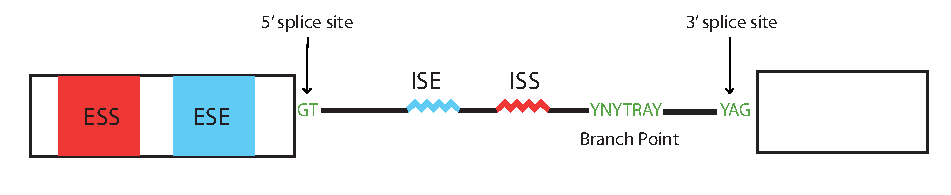
\includegraphics[width=\textwidth]{splicing_motifs}
    \caption[Cis-acting splicing motifs in eukaryotes]{Cis-acting splicing motifs in eukaryotes shown in an exon-intron-exon junction. The acceptor and donor dinucleotides are indicated at the 5' and 3' ends of the intron. ESE and ESS = exonic splicing enhancers and silencers. ISE and ISS = intron splicing enhancers and silencers. Y = pyrimidines.}
    \label{fig:splicing_motifs}   
  \end{figure}
AS is tightly regulated by several cis- and trans-acting factors. This tight regulation ensures splicing fidelity by correctly guiding the splicing machinery towards the target acceptor and donor splice sites, and by a complex interplay of splicing factors that promote and/or inhibit splicing (Figure \ref{fig:splicing_motifs}). Despite the apparent complexity of the splicing code \cite{Jaganathan2019-ah}, direct mutagenesis as well as computational approaches have elucidated several cis-acting sequence elements that guide the choice of splice sites and improve spliceosomal efficiency. These include exonic splicing enhancers (ESE), exonic splicing silencer (ESS), intronic splicing enhancers (ISE) and intronic splicing silencers (ISS). Splicing regulatory elements mostly work by recruiting various classes of trans-acting splicing factors to their target splicing sites. These factors either promote or hinder the recruitment of the spliceosomal complex. Most ESEs are bound by members of the serine/arginine rich proteins (SR proteins), which enhance the recruitment of several snRNPs necessary to initiate the splicing process (reviewed in \cite{Shepard2009-os}). The promotion of splicing is often countered by the recruitment of heterogenous nuclear ribonucleoproteins (hnRNPs) to ESS, which often block the recruitment of the splicing machinery \cite{Geuens2016-yz}. The disruption of this tight regulation underpins several diseases. Spinal muscular atrophy, a debilitating motor neuron disease, is caused by exon 7 skipping in \textit{SMN1}. Exon 7 skipping is caused by a single nucleotide substitution that alters the ESE sequence and results in a non-functional \textit{SMN1} protein isoform \cite{Monani1999-vf}.\\

\subsection{Cataloguing alternative splicing: progress and gaps}
Recent efforts to catalogue the human transcriptome have shown remarkable diversity of alternative isoforms. For example, the Reference Sequence (RefSeq) project uses a multi-modal approach to identify a high-confidence set of splice variants for each gene for thousands of organisms including over 770 mammalian transcriptomes \cite{OLeary2016-ci}. Manual curation by experts in addition to high-quality RNA-seq, proteomics, and histone marker datasets are used to build a bona fida set of gene splice variants. This effort has led to a 100-fold increase in the number of identified transcripts across mammalian species, from approximately 126,000 transcripts in 2003 to over 12 million transcripts in the latest RefSeq release (September 2023; \cite{refseq_ftp}). \\

Despite these significant advances, our knowledge of the distribution and roles of these splice variants in different tissues and cell types remains heavily underexplored. The evidence supporting the tissue-specificity of AS is contradictory. Wang et al. estimated that between 55-83\% of AS events vary between tissues in 15 studied human tissues and cell lines \cite{Wang2008-yg}. Others have shown that the majority of genes have a single dominant protein isoform in most tissues \cite{Ezkurdia2015-iv,Gonzalez-Porta2013-il}. However, many of these studies suffer from either biased transcriptomic or proteomic profiling methods or a small number of tissues. Fewer studies have attempted to systematically catalogue splice variants in an unbiased manner. In comparison, overall levels of gene expression in diverse tissues are being extensively studied by collaborative initiatives such as the Human Cell Atlas \cite{hca_resources}. Similar collaborative efforts that catalogue splice variants in an unbiased manner are warranted given the central role of AS in human health and disease.


\subsection{Technological limitations}
Several factors may explain why AS has received less attention compared to other transcriptional processes. The combinatorial nature of AS means that up to thousands of transcripts can be produced from the same genetic code. This poses several technological and analytical challenges. Most large-scale RNA-seq projects so far have relied on short-read sequencing to study the transcriptome. The complexity of AS patterns therefore makes it difficult to distinguish between distinct isoforms using 50-150 bp reads, as exonic sequences significantly overlap in alternative transcripts \cite{Lacroix2008-wq}. In principle, it is not possible to assign short reads to specific isoforms. \\

Creative technological and analytical techniques have been developed to assign short reads to their original transcript molecule. For example, Hagemann-Jensen et al. have recently applied a tagmentation strategy to map reads originating from the internal segments of gene bodies to UMI-tagged 5' reads. Using this technique, 30-50\% of reconstructed molecules were successfully assigned to a specific isoform \cite{Hagemann-Jensen2020-ob}. Additionally, computational techniques to reconstruct full isoforms from short reads have been developed. For example, Cufflinks relies on a reference transcriptome to estimate the most likely proportion of each splice variant given the observed RNA-seq reads \cite{Trapnell2012-zh}. Another method called rMATS estimates isoform proportions from the reads that support each type of AS event such as exon skipping and inclusion \cite{Shen2014-bq}. What these computational methods have in common is that they provide probabilistic estimates of isoform proportions, which underscores the inherent difficulty of obtaining a complete picture of isoform diversity from short-read RNA-seq experiments \cite{Shen2014-bq,Katz2010-kl}. These challenges explain why transcriptomic studies have focussed mostly on overall levels of gene expression, whose experimental and computational analysis workflow are more mature and suffer from less quantification uncertainty.

\subsection{Leafcutter as an intron-centric AS quantification method}
\begin{figure}
    \centering
    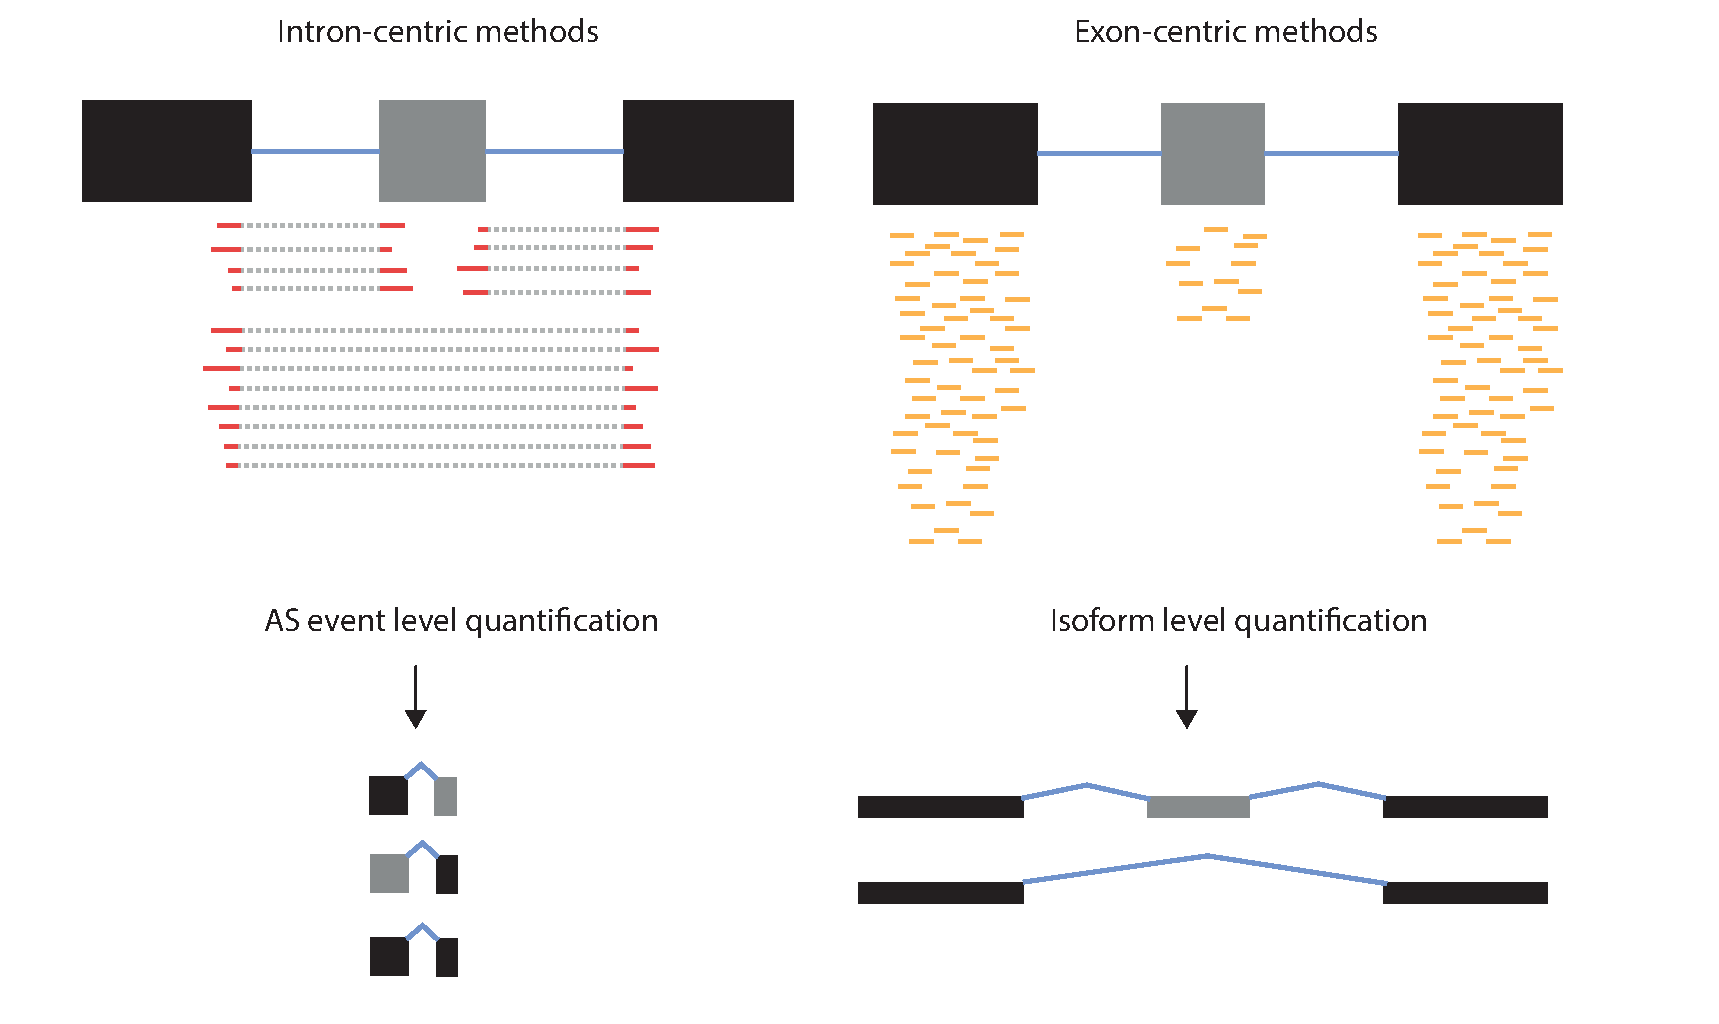
\includegraphics[width=\textwidth]{intron_exon_centric}
    \caption[Broad classification of alternative splicing quantification methods]{AS quantification methods are broadly classified into exon-centric methods and intron-centric methods. Exon-centric methods use exonic RNA-seq reads to estimate isoform abundance. Intron-centric methods such as Leafcutter quantify individual AS events. }
    \label{fig:intron_exon_centric}   
  \end{figure}
AS quantification methods can be broadly divided into exon-centric and intron-centric methods. Exon-centric methods use exonic reads or a combination of exonic reads and reads that span two splice junctions (split reads) to infer isoform-level counts. These methods are heavily dependent on a known reference transcriptome, with some improvements to increase their ability to identify novel splice junctions \cite{Vaquero-Garcia2016-dv}. Their underlying assumption is that the relative abundance of exonic reads reflects the proportions of the unobserved isoforms. Conversely, intron-centric methods are based on the principle that AS proceeds in a step-wise fashion, where introns are excised from pre-mRNA. Instead of quantifying AS using exonic reads, intron-centric methods use observed split reads at each splice junction to directly quantify local AS events (Figure \ref{fig:intron_exon_centric}). The obvious advantage of intron-centric methods is that they provide less uncertain estimates of AS events as they do not attempt to provide probabilistic isoform-level quantifications. Moreover, they are able to detect novel splice junctions as they do not rely on a reference transcriptome to reconstruct isoforms. However, this comes at the cost of precision and interpretability. By definition, split reads that span exon-intron-exon junctions are less abundant than exonic reads. Consequently, intron-centric quantification methods such as Leafcutter build their AS quantification using many fewer reads than exon-centric methods such as MAJIQ, rMATS, or Cufflinks. Moreover, the interpretation of local AS events is usually less straightforward. Local AS events reflect local intron excision steps at each exon-intron-exon junction, but it is often unclear how different intron excision events relate to one another. \\

Leafcutter is an example of intron-centric AS quantification methods that use split reads to quantify local intron excision decisions. In its first pass, Leafcutter starts by pooling all observed split reads in all samples to identify a set of high-confidence intron excision events. In a second pass, Leafcutter counts per-sample the number of split reads that map to each intron identified in the first pass. To improve interpretability, Leafcutter then organises individual intron excision events into undirected graph structures called \textit{intron clusters}. Nodes represent local intron excision events which are connected by edges. The Leafcutter algorithm connects two nodes (i.e. introns) if they share a 5' or 3' splice site. The overall Leafcutter procedure results in functionally connected intron cluster where any two connected introns share an acceptor or donor splice site. Within each intron cluster, intron usage is then quantified as the proportion of all split reads that map to each individual intron. This final quantification is performed separately for each RNA-seq sample and the result is a matrix of intron usage ratio for all study samples. 



\subsection{Mapping sQTLs}

Given the complex regulatory network that underpins AS regulation, understanding the impact of genetic variation on AS patterns paves the pathway to understand the impact of AS dysregulation on human health. Moreover, understanding how AS patterns are regulated in relevant contexts can help us better understand the impact of disease-associate genetic variant on the transcriptome. Similar to expression QTLs, where genetic variants associated with gene abundance are mapped, AS quantifications can be used as a molecular trait to uncover the genetic determinant of AS (splicing QTLs; Figure \ref{fig:leafcutter_conceptual}).\\

\subsubsection{General outline of QTL mapping}
QTL mapping pipelines are relatively well-established. Typically, a QTL analysis pipeline starts by obtaining an adequate number of samples where a quantitative molecular phenotype of interest is assayed (e.g. gene expression). Initial quality control steps are applied to ensure that experimental issues such as sample mixups are addressed. For transcriptomic studies, the first step after initial QC is to align NGS short reads to a reference genome. To extract quantitative molecular features from aligned reads, a quantification method is applied. The quantification method of choice usually depends on the research question of interest. For example, overall levels of gene expression are quantified using methods that count all short reads that map to each gene, and provide a gene count matrix. Similarly, methods that quantify AS provide an isoform-level or AS-event-level quantification. At this stage, another round of QC is often needed to ensure that low-quality features are removed from subsequent QTL mapping steps. Again, this QC step depends on the molecular QTL of interest. For example, it is important to remove introns detected in a small number of individuals, as tiny individual variations in intron usage can result in spurious sQTL associations. \\

With a post-QC feature matrix, QTL mapping follows a number of standard steps. The most important step before QTL mapping is to ensure that the molecular feature is properly normalised. Normalisation ensures that features conform to the assumptions of a linear regression model: homoskedasticity and normal distribution. These two assumptions are not only prerequisites of linear regression, but also ensure that effect sizes can be interpreted apppropriately. First, heteroskedasticity occurs when the variance of the predicted variable (i.e. feature) is not equal for different values of the independent variable (i.e. different genotypes). Quantile normalisation is one of the most widely used approaches to ensure that a molecular feature has equal variance across all samples in a study, satisfying the homoskedasticity condition. Second, an inverse normal transformation is applied to each sample to ensure that the feature is normally distributed.\\ 

Each molecular QTL can be tested for association with genetic variants in \textit{cis} or in \textit{trans}. Typically, cis-QTL mapping tests the association between a molecular feature and all nearby variants (e.g. within a 1 mbp window), while trans-QTL mapping tests the association between a molecular feature and distant genetic variants (e.g. > 5mbp or on other chromosomes). Cis-QTL mapping is more common as it requires less statistical power to detect an association, owing to the much smaller set of tested variants. For each molecular feature, thousands of genetic variants are usually tested. Compared to GWASes where all variants are tested genome-wide, the number of tests performed in QTL mapping is highly dependent on each individual feature. Setting a significance threshold therefore requires a different approach to a traditional GWAS significance threshold. A common approach to correct for multiple testing is to perform a permutation test between genotypes and features. The genotype-feature mapping is permuted hundreds or even thousands of times and association tests are performed again, resulting in a null distribution of association statistics. The real association statistic is then compared to the null distribution to obtain an adjusted association statistic. This layer of multiple testing correction accounts for the thousands of variants tested for each molecular feature. Another layer of multiple testing correction is applied to account for the thousands of molecular features tested in the QTL study. \\

\subsubsection{Special considerations in sQTL mapping}
Although the steps outlined above are standard for all QTL studies, there are a few conceptual and methodological differences between splice and expression QTL mapping. Depending on the AS quantification method, the interpretation of sQTLs can vary. sQTLs discovered using isoform abundance as a molecular trait are the easiest to interpret. A significant isoform-level sQTL would be defined as a genetic variant that increases or decreases a particular transcript abundance. This interpretation is less straightforward when AS is quantified at the AS event level. When intron usage ratios are used as quantitative trait, a significant sQTL can be defined as a variant that changes the proportion of a particular intron within its intron cluster. Therefore, when sQTLs are mapped using intron usage ratios, it is often helpful to examine the effect of the discovered genetic variant on all neighbouring AS events to build a more complete picture of the splicing event under investigation. For example, in Figure \ref{fig:intron_exon_centric}, upon examination of all three AS events in the left-hand panel, it becomes clear that the identified AS events represents an exon inclusion/skipping event. Additionally, it is important to note that different AS events are often highly correlated. This is because intron usage ratios within an intron cluster always add up to 1. Therefore, a genetic variant that leads to increased usage of one intron also leads to decreased usage of one or more other introns. As a result, multiple significant sQTLs within a single intron cluster do not necessarily represent distinct regulatory effects, but rather highly correlated measurements. 
\begin{figure}[H]
    \centering
    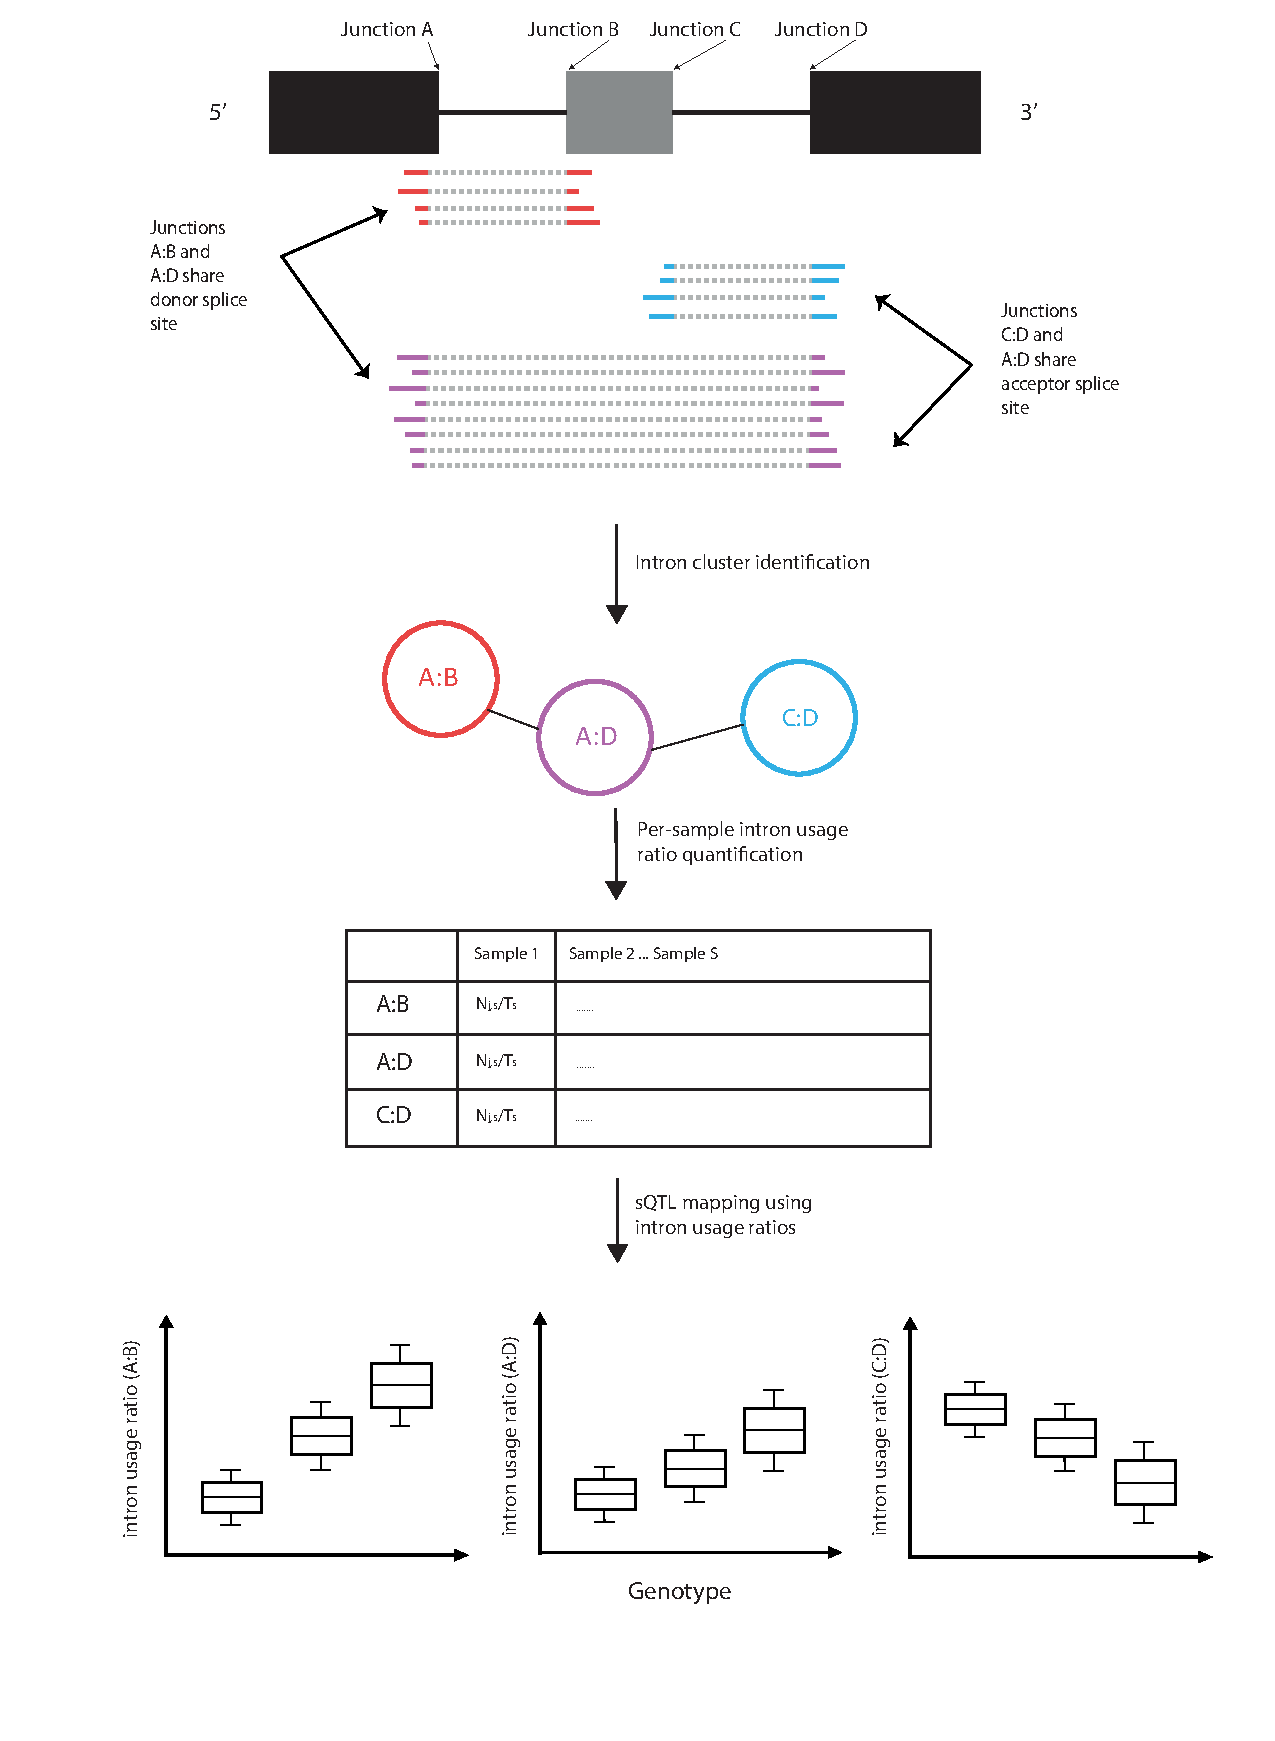
\includegraphics[width=\textwidth]{leafcutter_conceptual}
    \caption[Conceptual overview of splicing quantitative trait loci mapping using intron usage ratios]{Conceptual outline of sQTL mapping using intron usage ratios as quantitative traits. Intron clusters are identified from all pooled samples in a study. Quantification is then performed for each intron per sample. For a sample $S$, and an intron cluster with total number of reads $T_{S}$, the intron usage ratio for intron $j$ is defined as $\frac{N_{j,S}}{T_{S}}$. Intron usage ratios are then used as quantitative trait to map sQTLs in \textit{cis} with neighbouring genetic variants.}
    \label{fig:leafcutter_conceptual}   
  \end{figure}

\subsection{Comparing QTL effects in multiple contexts}
A long-standing question in QTL studies is how gene expression is genetically regulated in different tissues, cell types and environmental contexts. Answering this question is important to understand which transcriptomic effects of genetic variation are shared or distinct in different biological contexts. Context-dependence of QTL effects has often motivated multi-tissue QTL studies, with the assumption that profiling QTL effects in different contexts can draw a more complete picture of gene expression regulation. For example, in a comparison of eQTL effects between CD4+ T-cells and monocytes, Raj et al. \cite{Raj2014-xw} found that at least 42 genes had opposing eQTL effects in the two cell types. In line with this, Peters et al. \cite{Peters2016-zk} found that 87 genes had discordant eQTL effects in five different immune cell types. Although these dramatically discordant examples of genetic regulation represent a minority of QTL effects, the question of which QTL effects are modulated in a more subtle manner in different contexts remains relevant \cite{Fairfax2012-ur,Lee2014-zo,Umans2021-fv,Van_de_Geijn2020-zn,Gamazon2018-uz}.\\

Assessing the sharing of QTL effects in different treatment groups is non-trivial. In most QTL studies, QTL discovery is carried out separately for different treatment groups. This means that incomplete power may cause truly shared QTL effects to appear non-significant in some groups simply by chance. Direct comparison of statistical significance between different groups is therefore likely to overestimate the number of distinct QTL effects. To address this issue, several methods that probabilistically model effect sizes were developed \cite{Flutre2013-sp,Li2018-kr,Sul2013-xm, Urbut2019-gf}. Earlier methods were inspired by fixed-effects meta-analysis methods, and started from the assumption that any given eQTL effect is shared across all conditions and sought to find statistical evidence to the contrary (i.e. context-specificity).\\

Later, methods that learn the data-driven correlation structure were developed. For example, multivariate adaptive shrinkage (mash) empirically learns the patterns of effect sharing in the dataset under study, and allows for arbitrary patterns of sharing between different groups. For example, QTLs derived from different brain regions are expected to have highly correlated effect sizes. Usually, this correlation structure is learned from a random unbiased set of QTL effects (i.e. non-significant QTLs). A Bayesian approach is then applied to re-estimate effect sizes for a desired set of QTL effects (e.g. significant QTL effects). The posterior effect sizes are then tested for evidence of effect size heterogeneity between different groups, taking the underlying data-driven correlation structure into account. The obvious advantage of mash is that the re-estimated effect sizes take into account the empirical correlation structure in the dataset. However, this also means that significant QTL effects' sharing may be overestimated when the null QTL effects are highly correlated among the treatment groups. As a result, this may hide truly context-dependent QTL effects simply because there is not enough statistical evidence to suggest heterogeneity of effect sizes. Additionally, when significant QTL effects are tested for condition-specificity, only the lead QTL SNP is used. In many cases, sharing of the lead QTL SNP does not necessarily mean that the underlying causal variant is shared between different conditions. It has been previously shown that comparing the lead SNP between different association signals can lead to the false conclusion that the effects under comparison are shared \cite{Liu2019-fv}. A better approach should leverage the linkage disequilibrium structure to assess if two association signals under comparison are likely to be shared or distinct. Nonetheless, mash can still be useful if the degree of QTL sharing is interpreted as an upper bound, rather than an accurate estimate of QTL sharing.\\


\subsection{Linking disease-associated GWAS loci to QTLs}
In addition to understanding gene regulation, a major objective of QTL studies is to dissect the effects of disease-associated loci in relevant tissues and cell types. The simplest approach is to test the replication of the lead GWAS SNP in the QTL dataset. It is often compelling to assume that a replicated SNP may indicate that both gene expression and disease risk are driven by the same variant. In fact, lead SNP comparison was commonly used to implicate effector genes at many disease-associated loci. However, this direct SNP comparison was found to result in many false positives \cite{Liu2019-fv}. Therefore, more robust methods to compare pairs of association signals were developed to fill this gap. Particularly, statistical colocalisation methods take into account the association signal of all variants in a region to make a conclusion about a pair of association signals. Although the true causal variant may not be genotyped or imputed in either of the association studies, its effect is tagged by other variants in linkage disequilibrium with the true causal variant. Colocalisation methods leverages the linkage disequilibrium in a given locus to make an inference about two association signals. The underlying assumption is that if the two association signals are consistent across the region, it is likely that the same variant is driving both signals. Therefore, colocalisation results are only valid when the LD pattern is similar between the two association signals under comparison. This assumption only holds if the two association signals being compared are derived from populations with matching LD structures, an important consideration when colocalisng signals from GWAS and QTL studies. Additionally, standard colocalisation approaches only test the hypothesis that a \textit{single} shared variant underpins the two association signals. Many QTL studies have shown that secondary and even tertiary association signals have been discovered for several genes \cite{macromap-eqtl,De_Klein2023-ku}, and the same observation applies to GWAS signals. Violations of the single causal variant assumption at loci with multiple causal variants will result in decreased power to detect true colocalisations. Therefore, extensions to standard colocalisation identify independent association signal in each of the two cohorts, before proceeding to perform colocalisation analysis for each of the identified signals. This approach has been shown to increase the number of colocalised signals detected \cite{Wallace2021-rv}.\\  


\subsection{Current status of sQTL studies}
Several studies have investigated the genetic regulation of alternative splicing. These studies include relatively fewer multi-tissue or multi-cell-type studies as well as single-tissue or single-cell-type studies. Notably, virtually all of these studies are bulk RNA-seq studies because the most widely used single cell RNA-seq methods capture only a few bps at the start or end of each RNA molecule. The imminent development of single-cell long-read RNA-seq methods is set to change this by allowing full-length RNA isoforms to be directly mapped at a single-cell level \cite{Dong2023-xs}. Still, bulk sQTL studies have taught us a few interesting insights. In this section, I will focus on two relevant aspects of the genetic regulation of AS: context-specificity and role of AS in complex disease risk.\\

The most diverse sQTL study to date is the GTEx consortium, where eQTLs and sQTLs were mapped across 49 human tissues from 70-700 individuals. GTEx tissues represent a heterogenous mix of different cell types, which makes an investigation of cell-type-specificity of alternative splicing difficult. However, GTEx was still useful understand the patterns of alternative splicing sharing across tissues. It was found that tissue sharing follow a U-shaped distribution, meaning that the majority of sQTL effects were either found in a small number of tissues (1-5) or shared across almost all tissues (45-49 tissues). This pattern was less evident for eQTL effects, which suggested that sQTLs are generally more tissue-specific than eQTLs \cite{The_GTEx_Consortium2020-gg}. However, it is difficult to disentangle the effect of different statistical power in different tissues from true tissue specificity. Indeed, a subsequent re-analysis of the GTEx splicing data (Garrido-Martín et al. 2021 \cite{Garrido-Martin2021-sk}) found that sQTL effects with large effect sizes, which are more readily discovered with small sample sizes, tend to be shared between tissues, and vice versa. When Garrido-Martín et corrected for sample size differences between various tissues, they found that brain, testis, liver and skeletal muscles had large numbers of tissue-specific sQTLs. These observations show that sQTL effects, especially one with smaller effect sizes, show patterns of tissue-specificity. \\

sQTLs were also shown to contribute significantly to complex disease risk in two major meta-analysis of brain and immune cell sQTL studies. Qi et al. 2022 \cite{Qi2022-iz} mapped sQTLs from over 2800 RNA-seq samples, and discovered thousands of significant sQTLs and eQTLs. The availability of both eQTLs and sQTLs allowed them to compare their contribution to complex disease risk. To this end, they quantified the contribution of both sQTLs and eQTLs to the SNP heritability of 12 brain-related complex diseases, and showed that both molecular QTLs contributed roughly equally to disease heritability. Moreover, when they performed colocalisation with disease-associated loci, they found that both molecular QTLs implicated distinct gene sets. This finding was also mirrored in another eQTL and sQTL meta-analysis of 18 different immune cell types (Mu et al. 2021 \cite{Mu2021-ar}). Mu et al. compared the contribution of eQTLs sQTLs in different cell types to immune disease risk. Similar Qi et al., they also found a significant contribution of sQTLs, as measured by the number of loci that colocalised with high confidence with disease-associated loci. For many complex traits, this contribution often exceeded the contributionof eQTLs.\\

\subsection{Contribution of this thesis}
In the first part of my thesis, I will use iPSC-derived macrophages (MacroMap) to address the previously mentioned two aspects of alternative splicing regulation: the context specificity of AS regulation, and the contribution of AS to immune-mediated disease risk. Although the GTEx sQTL results indicate that AS regulation may be tissue specific, it does not provide an account of which genes are alternatively spliced in a cell-type or context-specific manner. This is mainly because GTEx tissues are a mixture of several cell types. Moreover, even fewer studies addressed the question of whether cells respond to environmental stimuli at the AS level. For example, do cells respond to pathogens by altering isoforms in genes relevant for microbial clearance? What role does the genetic regulation of AS play in such a response?\\

As part of the MacroMap project, iPSC-derived macrophages from over 200 individuals were exposed to a wide range of stimuli. I will describe how I used genotype and RNA-seq data to study the patterns of alternative splicing in different stimulation conditions, and to identify genetic variants that regulate alternative splicing in different macrophage environmental contexts. I will describe examples of the widespread differential splicing between stimulated and unstimulated macrophages, often implicating core innate immune response pathways. Additionally, I will show that alternative splicing regulation is often context-dependent, and that a considerable proportion of sQTL effects are modulated upon exposure to environmental stimuli. Finally, I will describe how I linked hundreds of immune disease loci to alternative splicing changes in macrophages and give examples of alternative splicing dysregylation by disease-associated risk loci. An important insight of this work is that in the context of IMD risk, the dysregulation of alternative splicing is at least as important as the dysregulation of overall levels of gene expression. Finally, I will highlight the potentially important role of lowly-used splice junctions in immune disease risk, a role that has been, so far, under-appreciated.

\section{Part II: sub-phenotype GWAS}
\subsection{Genome-wide association studies}
Complex disease risk is determined by a multitude of genetic and environmental factors. Over the last 18 years, genome-wide association studies (GWAS) have revolutionised our understanding of the genetic component of complex disease risk. The Wellcome Trust Case Control Consortium (WTCCC) ushered the era of GWAS studies by designing large-scale case-control cohorts for several common disorders. Since then, the case-control experimental design has been exploited in thousands of GWAS studies to uncover the genetic determinants of cardiovascular, metabolic, immune-mediated, musculoskeletal, neurological, and gastrointestinal diseases. In most cases, these cohorts are built through collaborative efforts between recruitment centres, hospitals and other healthcare facilities and research centers that identify disease cases and controls, and provide biological samples needed to conduct array-based or exome-based genotyping. The continuous growth of sample sizes has increased our ability to detect genome-wide significant loci associated with disease risk. These efforts have also revealed the extensively polygenic nature of most complex diseases, whereby hundreds of genetic loci increase or decrease disease risk with small effect sizes. The complexity of the genetic architecture of most common disease has initially made it more challenging to draw biological insights. Although most GWAS results were initially puzzling, over the last few years massive GWASes have revealed biological insights about common diseases \cite{Xue2018-ni,Aragam2022-ep}. This increased understanding was facilitated by the availability of functional genomic datasets as well as methodological advances in linking genetic variants to biological functions. 

\subsection{Inflammatory bowel disease}
\subsubsection{Epidemiology and classification}
Inflammatory bowel disease (IBD) encompasses a group of immune-mediated disorders of the gut. IBD poses a considerable burden for healthcare systems globally. In 2017, IBD affected over 6.8 million individuals worldwide, with a rising global burden since at least the 1990s. IBD incidence shows notable geographical variation, with the highest incidence reported in North America, the UK and northern Europe. Moreover, IBD incidence has notably risen in countries that are becoming increasingly "westernised" in terms of their environmental risk factors, such as China and South Korea, consistent with a significant environmental contribution to IBD \cite{Ng2013-of}.\\

IBD is broadly classified into two broad categories based on radiological, clinical and endoscopic features: ulcerative colitis (UC) and Crohn's disease (CD), although 6-13\% are classified as IBD unclassified (IBDU) \cite{Thurgate2019-xj}. The two classes show differences in terms of disease behaviour and location, clinical manifestations and prognosis. UC inflammation occurs in a continuous manner and is often characterised by chronic mucosal inflammation and leukocyte infiltration \cite{Hendrickson2002-ky}. UC usually starts near the rectum and diffuses proximally to different parts of the colon. On the other hand, CD can affect any part of the GI tract from mouth to anus and is characterised by patches of inflammation (skip areas). Inflammation often extends beyond the gut mucosa involving the submucosa. CD most frequently occurs in the ileo-coecal region followed by isolated terminal ileal inflammation. Clinically, CD is a heterogenous disease characterised by a remitting-relapsing clinical picture. Most patients experience abdominal pain, rectal bleeding, and altered bowel habits. However, other clinical aspects of CD vary between patients and can often make the difference between favourable or unfavourable disease course and prognosis. Some CD patients experience relatively infrequent CD flares, with milder symptoms that respond well to treatment. Others experience more frequent episodes of severe GI symptoms. Severe CD patients also often develop transmural manifestations such as penetrating disease, fistulas and abscess as well as extraintestinal manifestation involving the eye, joints and/or other systemic manifestations. Although the majority of CD patients undergo surgery at least once over their lifetime, patients who have non-penetrating non-fistulising CD manifestations are less likely to require surgery \cite{Lewis2010-gx}. %Understanding the genetic determinants of the different clinical aspects of CD is therefore crucial for a more nuanced biological insight into what drives disease course. 



\subsubsection{Risk factors of IBD}
IBD is a complex disease, which is likely caused by an interaction of genetic, environmental, and lifestyle factors. IBD has often been described as an "industrialised nations" diseases, with higher prevalence in developed countries. Epidemiological studies have shown increasing prevalence of IBD in nations that are becoming increasingly industrialised. Interestingly, second-generation immigrants from low-prevalence countries have experienced increasing incidence of IBD \cite{Bernstein2008-ln}. These observations have linked IBD risk to "industrialised" lifestyle factors, whereby environmental and lifestyle factors common in industrialised countries are thought to contribute to IBD risk. These changes have led to reduced exposure to infectious agents, improved hygiene and sanitation, an increasingly sedentary lifestyle and increased consumption of processed foods, and foods rich with sugar and saturated fats.\\

Smoking is the best described lifestyle factor linked to IBD risk. Smoking has been shown to increase risk of CD and decreasing risk of UC. However, the mechanism of this paradoxical association between smoking and IBD is not completely understood \cite{Richardson2003-pd}.  Other non-dietary factors include oral contraceptive pill intake, which was shown to increase both CD and UC risk \cite{Cornish2008-rn}, and appendectomy which was associated with reduced UC risk \cite{Koutroubakis2000-qt}.\\

The effect of lifestyle choices and diet on IBD have been extensively studied, but the results are often difficult to assess. Exercise is known to boost immunity and decrease proinflammatory cytokines. However, the severity of IBD symptoms often impacts patients' physical activity, and studies linking exercise to IBD progression have been therefore confounded by IBD severity \cite{Rozich2020-ui}. Similarly, alcohol and coffee consumption were not conclusively linked to IBD development or progression \cite{Yang2019-gt}. However, obesity has been shown to independently worsen IBD behaviour and increase likelihood of relapse \cite{Jain2019-oy}. Diet composition also plays an important role in IBD risk. Its role has been attributed to the effect of diet on the gut microbiota composition and bahaviour. For example, a Japanese study has shown a significant association between IBD risk and total fat and unsaturated fat intake, fish and shellfish consumption, and $\omega$-3 and $\omega$-6 fatty acids \cite{Reif1997-li}.\\



\subsection{Inflammatory bowel disease genetics}
The genetic component of IBD has been recognised for over 70 years via family studies on twins. Family studies have shown that monozygotic twins are more likely to co-inherit IBD compared to dizygotic twins, often with similar disease behaviour and location \cite{Ng2012-mf}. Over the last decade, several GWASes have identified over 240 loci associated with IBD susceptibility \cite{Jostins2012-ig,De_Lange2017-re,Liu2015-bx,Luo2017-kx}. The largest IBD GWAS studies have focussed on discovering both common and rare genetic variants associated with IBD susceptibility. These studies have revealed several key mechanistic insights regarding the pathogenesis of IBD including autophagy, host-microbe interactions, intestinal innate immune response, and impaired epithelial barrier function \cite{Khor2011-td,Jostins2012-ig}. These pathways seem to converge on a IBD pathogenesis model whereby impaired intestinal permeability, leads to microbial infiltration into the gut mucosa. This microbial incursion activates intra-epithelial cells to initiate a cascade of innate and adaptive immune responses aiming to limit microbial spreading and restore normal barrier function. The integration of hundreds of genetic loci with functional genomic datasets have clearly improved our understanding of IBD susceptibility. However, given the clinical heterogeneity of IBD sub-types, understanding the genetic determinants of their different clinical aspects is crucial for a more nuanced biological insight into what drives disease course.\\

% Fewer GWAS studies have dissected other clinical aspects of CD. 
% CD is a heterogenous subtype of IBD characterised by a remitting-relapsing clinical picture. Most patients experience abdominal pain, rectal bleeding, and altered bowel habits. However, other clinical aspects of CD vary between patients and can often make the difference between favourable or unfavourable disease course and prognosis. Some CD patients experience relatively infrequent CD flares, with milder symptoms that respond well to treatment. Others experience more frequent episodes of severe GI symptoms. Severe CD patients also often develop transmural manifestations such as penetrating disease, fistulas and abscess as well as extraintestinal manifestation involving the eye, joints and/or other systemic manifestations. Although the majority of CD patients undergo surgery at least once over their lifetime, patients who have non-penetrating non-fistulising CD manifestations are less likely to require surgery \cite{Lewis2010-gx}. Understanding the genetic determinants of the different clinical aspects of CD is therefore crucial for a more nuanced biological insight into what drives disease course.\\

\subsubsection{Growing interest in the genetic determinantsof disease sub-phenotypes}
The evident success of GWAS studies in improving our understanding of CD biology has sparked the interest in using them to dissect complex disease sub-phenotypes. However, disease sub-phenotype GWASes have generally lagged behind susceptibility GWASes, due to the difficulty of obtaining deep phenotypic or longitudinal data for similarly large cohorts. It has been previously suggested that the same genetic variants drive both disease susceptibility and disease sub-phenotypes. However, evidence in relatively smaller sub-phenotype GWASes suggests that the genetic variants that underpin disease susceptibility and disease sub-phenotypes may also be distinct \cite{Iwaki2019-mf,Severe_Covid-19_GWAS_Group2020-rn}. Both paradigms raise interesting questions about the genetic architecture of disease susceptibility and sub-phenotypes. Under the former paradigm, it will be particularly important to understand the relationship between the effect of each variant on susceptibility and sub-phenotype risks. For example, for a given variant associated with both disease sub-phenotype and susceptibility, is the susceptibility risk truly driven by sub-phenotype risk? As sub-phenotype GWASes become more commonplace, it will be particularly interesting to compare the effects sizes of each variant on both susceptibility and disease sub-phenotypes. This may lead to better stratification of disease risk based on distinct sub-phenotype risk profiles. Under the latter paradigm, it is important to understand which distinct biological pathways are involved in disease sub-phenotypes risk and how they interact with disease susceptibility pathways. For example, fistulising CD has been hypothesised to originate as an epithelial-to-mesenchymal transformation, whereby stationary epithelial cells gain migratory features. Is this transformation accelerated by the impaired intestinal barrier and subsequent immune activation that likely underpins CD susceptibility?\\

The genetic architecture of CD sub-phenotypes has been explored in a number of studies. Longitudinal and deep phenotypic data from CD cohorts of thousands of patients were used alongside genetic data to map genetic variants associated with disease location, behaviour, surgery and prognosis. Because these studies are considerably less powered than susceptibility GWASes, they have only given an initial glimpse into the genetic architecture of CD sub-phenotypes. Therefore, it is still not possible to draw a conclusive answer to the question whether or not CD susceptibility and sub-phenotypes share genetic underpinnings. In the rest of this section, I will focus on two studies by Cleynen et al. 2016 \cite{Cleynen2016-ha} and Lee et al. 2017 \cite{Lee2017-tl} as notable examples of CD sub-phenotype GWASes. \\

Cleynen et al. \cite{Cleynen2016-ha} used 11 years of longitudinal data from approximately 17,000 CD patients to study the genetic determinants of CD sub-phenotypes. They performed several within-case GWASes of CD age-at-diagnosis, location, behaviour and surgery. Across all their CD analyses, they found three genome-wide significant loci at \textit{MST1} and \textit{NOD2} as well as an MHC association. Both the MHC and  \textit{NOD2} loci were associated with ileal versus colonic disease and with a penetrating (B3) versus inflammatory or stricturing disease (B1 or B2). Despite the small number of genome-wide significant loci, the authors built IBD polygenic risk score to compare individuals with different disease locations and behaviours. The main insight from their work was the rejection of the binary classification of IBD into CD and UC. Based on a polygenic risk score (PRS) comparison between individuals with different disease locations, they proposed a novel classification which places ileo-colonic CD as an intermediate form between ileal CD and UC. \\

Based on the discovered loci, the genetic relationship between CD susceptibility and CD sub-phenotypes is difficult to assess. For example, the \textit{NOD2} lead variant (rs2066847) is a frameshift variant that has been previously associated with CD susceptibility in several studies \cite{Barrett2008-lg,Jostins2012-ig} (P-value=$6\times10^{-209}$ in Jostins et al. data). However, the lead MHC variant (rs6930777) was not genome-wide significant in any CD susceptibility GWAS (source: GWAS catalogue accessed in November 2023). \\

% \begin{table}[]
%   \caption{Genome-wide significant loci associated with CD behaviour (B1 versus B2/B3) and CD location (ileal versus colonic) from Cleynen et al. 2021. CD susceptibility associations were obtained from the GWAS catalogue accessed in November 2023. N/A means no CD susceptibility association was available because none passed the minimum P-value threshold. N/R means association statistic was not reported.}
%   \label{tab:cleynen_gws}
%   \begin{tabular}{|l|l|l|l|l|l|l|l|}
%   \hline
%   SNP       & CD behavior P-value  & CD behaviour OR  & CD location P-value  & CD location OR   & CD susceptibility P-value & CD suscptibility OR & CD susceptibility study \\ \hline
%   rs6930777 & $2\times10^{-3}$     & 0.89 (0.82-0.96) & $8.13\times10^{-23}$ & 0.58 (0.52-0.65) & N/A                       & N/A                 & N/A                     \\ \hline
%   rs2066847 & $5.73\times10^{-10}$ & 1.31 (1.21-1.42) & $1.01\times10^{-35}$ & 2.50 (2.14-2.92) & $6 \times10^{-209}$       & N/R                 & Jostins et al.          \\ \hline
%   \end{tabular}
%   \end{table}
Comparatively, Cleynen et al. had a much smaller sample size than many CD susceptibility GWASes. The growth of sub-phenotype GWASes' sample sizes will enable a more systematic comparison of genome-wide significant associations of CD susceptibility and sub-phenotype variants. However, their PRS comparison may give a clue that may contribute to answering this question. The PRSs they built to compare different IBD forms were based on lead variants from all known IBD susceptibility loci. The ability of these PRSs to distinguish "macroscopic" features of IBD (e.g. CD versus UC or ileal versus colonic CD) lends support to the hypothesis that the genetic architectures of susceptibility and location are not entirely distinct. It is worth noting that the differences in PRS distribution between these groupings were quite small, but this could also be attributed to the low predictive power of PRSs in general.\\

A later study by Lee et al. \cite{Lee2017-tl} showed that the genetic determinants of CD prognosis were largely distinct from CD susceptibility variants. Lee et al. performed a within-case GWAS between two CD subpopulations at opposite ends of the prognosis spectrum. Poor prognosis individuals were defined as patients who experienced frequent CD flares that did not respond to treatment with immunomodulators and/or surgery. Good prognosis patients were defined as CD patients who showed good long-term response to treatment. Their analysis found four genome-wide significant loci in \textit{FOXO3} and \textit{XACT}, an intergenic locus in \textit{IGFBP1}-\textit{IGFBP3}, as well as an MHC association. These association were not found to be associated with CD susceptibility in any previous CD GWAS studies. Additionally, the authors found no evidence of genome-wide genetic correlation between CD susceptibility and CD prognosis, although it has to be noted that CD prognosis GWAS may have been underpowered to detect a significant genetic correlation ($r_{g}=-0.51$; P-value=0.12). Unlike Cleynen et al., these lines of evidence support the alternate hypothesis that the genetic architectures of CD susceptibility and CD prognosis, an example of a CD sub-phenotype, are distinct. Interestingly, a recent GWAS of multiple sclerosis progression reported a similar observation. The authors compared the long-term cognitive outcomes of MS patients with the highest and lowest MS PRSs, and found that PRSs did not differentiate between individuals with poor versus good MS prognosis \cite{ms_susceptibility}. Similarly, a GWAS of epilepsy prognosis concluded that it is unlikely that epilepsy susceptibility variants affect epilepsy prognosis \cite{Speed2014-lz}.\\

At this stage of CD sub-phenotype GWASes, it is perhaps too early to answer the question conclusively, since very little is known about the biological mechanisms behind each CD sub-phenotype. This is set to change as large-scale IBD resources grow and enable well-powered sub-phenotype GWASes that give us a better understanding of the biology behind each CD sub-phenotype. \\


\subsection{Contribution of this thesis to sub-phenotype understanding}
In my thesis, I attempt to identify the genetic variants associated with perianal CD, as an example of a CD sub-phenotype. pCD is a severe CD sub-phenotype characterised by abscess and fistula formation around the anal region. Collaborative efforts have enabled detailed clinical phenotyping of thousands of CD patients, including information on perianal symptoms. I describe a GWAS meta-analysis between CD patients with and without pCD in two IBD patient cohorts (UK IBD Genetics Consortium and IBD BioResource). As a follow-up, I also studied the genetics of sporadic perianal manifestations in the general population. Although perianal symptoms are highly enriched among CD patients, perianal fistulising disease also occurs sporadically, often not accompanied by CD. To understand the genetics of the two types of perianal manifestations, I performed an additional GWAS meta-analysis between individuals who report sporadic perianal disease and healthy controls in the UK Biobank and FinnGen. This meta-analysis revealed several genome-wide significant loci associated with sporadic perianal manifestations. My initial assessment shows that none of these loci replicate in the pCD meta-analysis, possibly suggesting distinct mechanisms driving both types of perianal manifestations. Overall, the aim of chapters 3 and 4 of my thesis is to study perianal manifestations as an example of a CD sub-phenotype, both in the context of CD and in its sporadic forms in the general population. 





% Moreover, investigating the interaction of these factors with the immune system has led to the "hygiene hypothesis".  

% \subsubsection{Colocalisation}

% \subsubsection{Other approaches}

% % Statistical modelling of effect sizes tests the alternative hypothesis that a given effect size is significantly different in one or more treatment groups. Different methods test this hypothesis in different ways. Earlier methods were inspired by fixed-effects meta-analysis approaches and 
% % The complex regulatory network of cis-acting elements and trans-acting factors suggests that regulatory errors can arise 

% % Since the 1970s, alternative splicing (AS) has emerged as an important post-transcriptional modification. AS has been shown to remarkably increase the coding potential of an otherwise fixed repertoire of genes. Through diversification of the transcriptome, AS contributes to phenotypic complexity in higher organisms. Previous work has shown that AS is more prevalent in higher eukaryotes compared to lower eukaryotes, and in vertebrates compared to invertebrates (10.1038/nrg2776). Our appreciation of the role of AS has also changed over time. Today, we know that 95% of multi-exonic genes are alternatively spliced, compared to an estimate of only 5-35% shortly after the Human Genome Project (https://www.hindawi.com/journals/ijeb/2012/596274/; https://www.ncbi.nlm.nih.gov/pmc/articles/PMC2443848/). 


% \subsection{why we need qtl studies}
% \subsection{why molecular qtls are context dependent - same dna - different gene expression}
% \subsection{why is it important to understand disease-associated variants in a relevant context}
% \subsection{the variety of molecular QTLs: caQTLs, histone marker QTLs..etc}
% \subsection{Most studies have focussed on overall levels of gene expression}